\documentclass[border=15pt, tikz]{standalone}
\usepackage[T1]{fontenc}
\usepackage[utf8]{inputenc}
\usepackage{tikz}
\usetikzlibrary{positioning, arrows.meta, decorations.pathreplacing, calc, fit}
\definecolor{clrattention}{HTML}{45B7D1}
\definecolor{clrattention_alt}{HTML}{96E6F0}
\definecolor{clrffn}{HTML}{F97068}
\definecolor{clrnorm}{HTML}{FFD93D}
\definecolor{clrembed}{HTML}{6BCB77}
\definecolor{clrresidual}{HTML}{4D96FF}
\definecolor{clroutput}{HTML}{C084FC}
\definecolor{clrspectral}{HTML}{22D3EE}
\definecolor{clrphysics}{HTML}{FB923C}
\definecolor{clrborder}{HTML}{334155}
\definecolor{clrtext}{HTML}{1E293B}
\definecolor{clrgroup_frame}{HTML}{94A3B8}
\definecolor{clrgroup_fill}{HTML}{F1F5F9}
\begin{document}
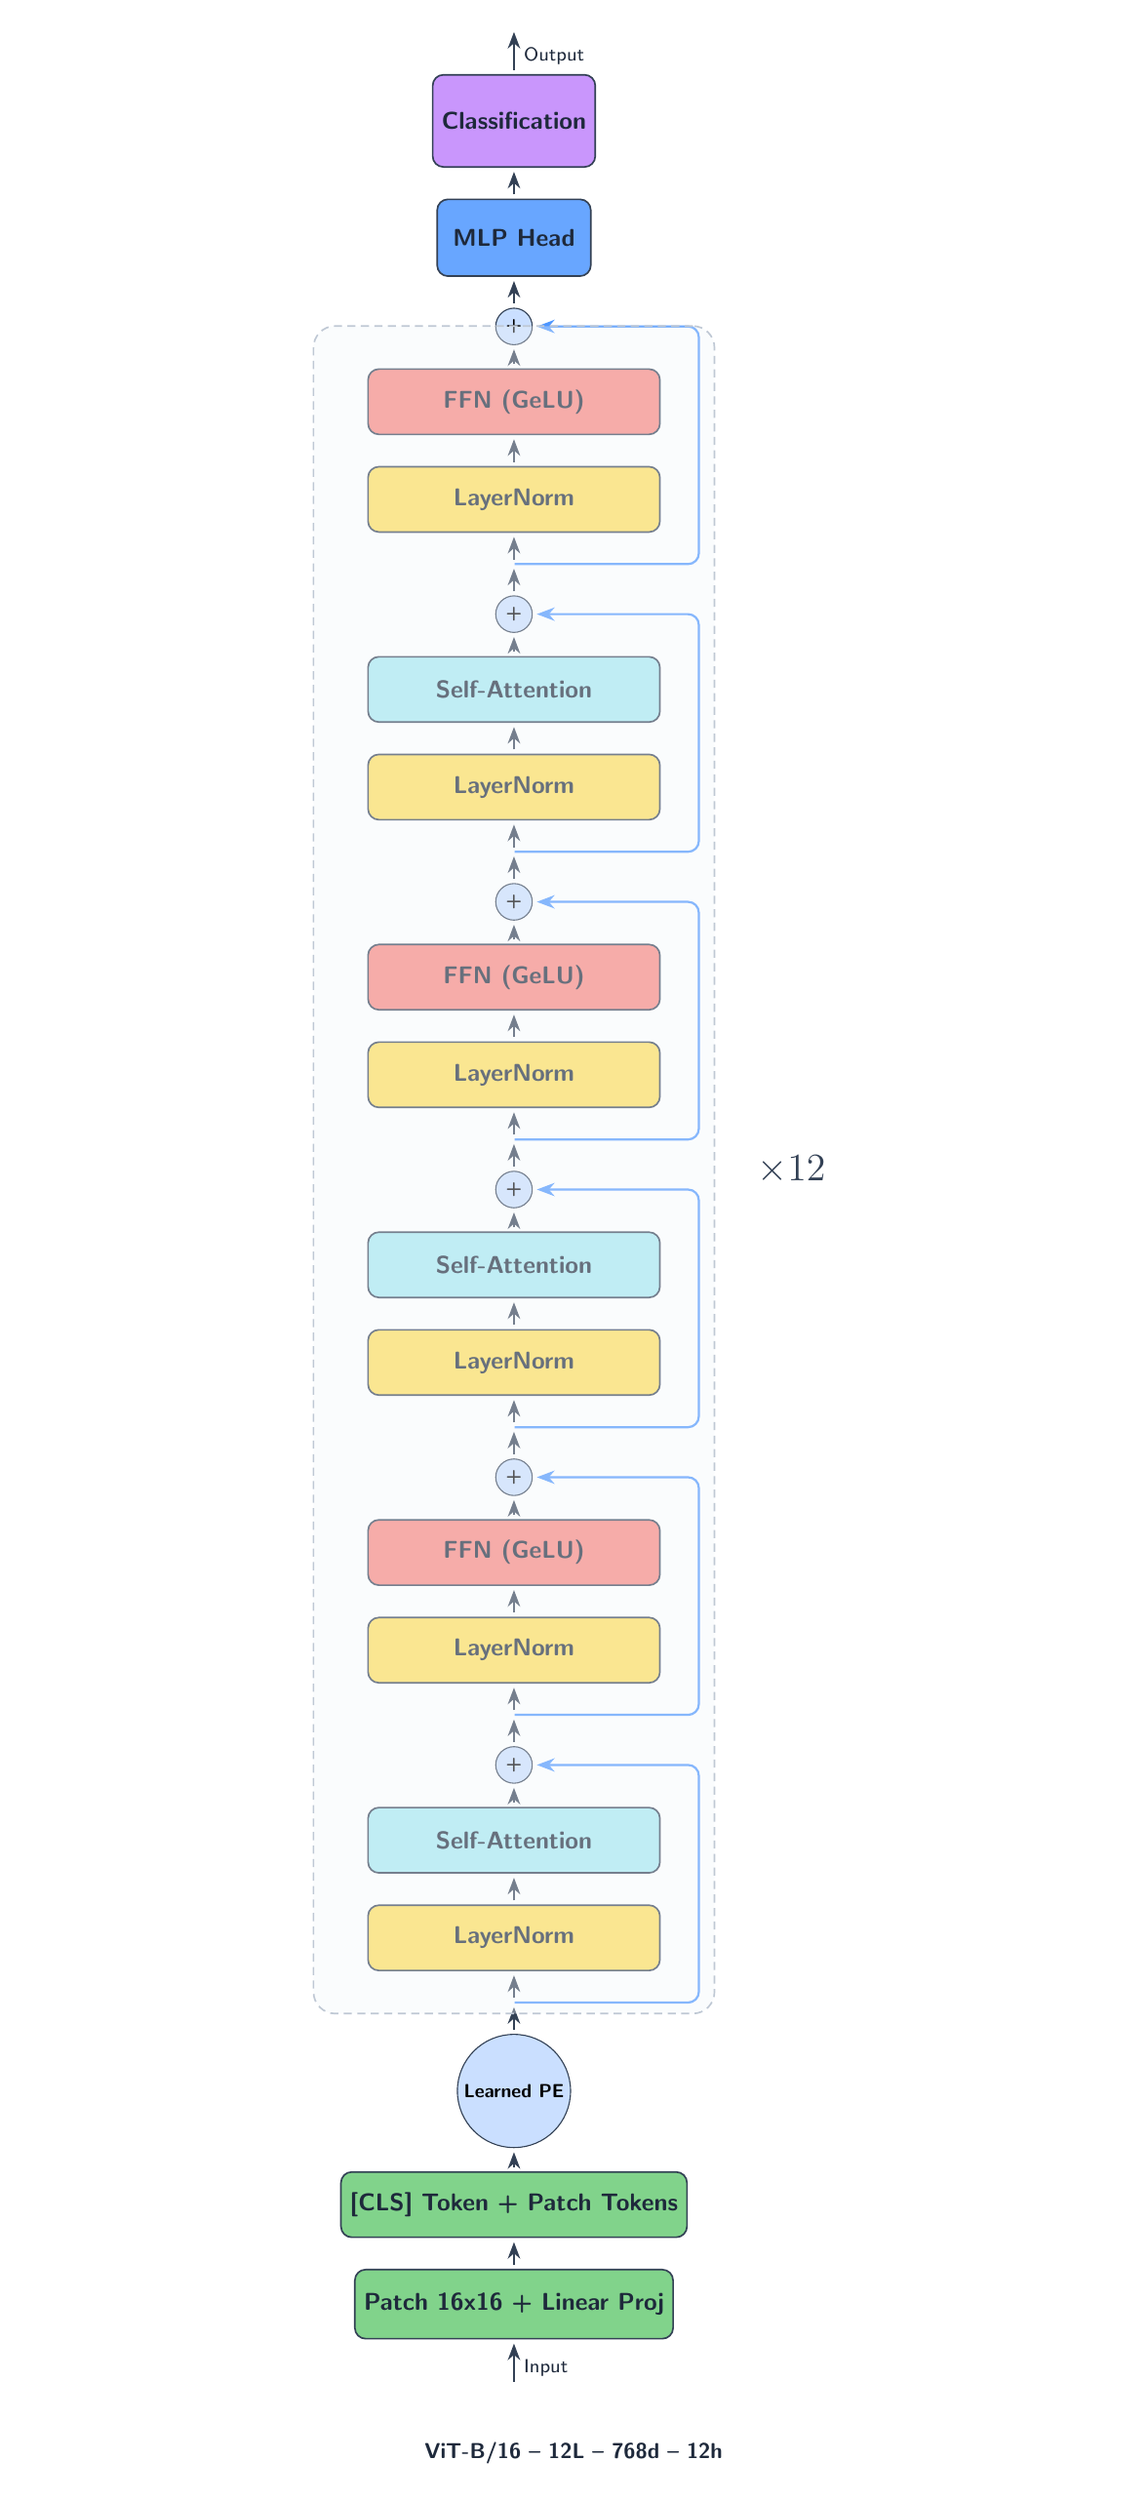
\begin{tikzpicture}[
    >=Stealth,
    every node/.style={font=\sffamily},
    block/.style={draw=clrborder, rounded corners=4pt, minimum width=3.8cm,
                  minimum height=0.85cm, font=\sffamily\small\bfseries,
                  text=clrtext, line width=0.6pt},
    arrow/.style={->, thick, color=clrborder, line width=0.7pt, shorten >=1.5pt, shorten <=1.5pt},
    skiparrow/.style={->, thick, color=clrresidual, line width=0.8pt, rounded corners=4pt, shorten >=1.5pt},
    label/.style={font=\sffamily\scriptsize, text=clrtext},
    subtitle/.style={font=\sffamily\footnotesize, text=clrtext},
]
\node[block, fill=clrembed!85, minimum width=4.0cm, minimum height=0.9cm, text=clrtext] (n_1) at (0,0) {Patch 16x16 + Linear Proj};
\node[block, fill=clrembed!85, minimum width=4.0cm, minimum height=0.85cm, text=clrtext, above=0.4cm of n_1] (n_2) {[CLS] Token + Patch Tokens};
\node[circle, draw=clrborder, fill=clrresidual!30, inner sep=2pt, font=\sffamily\scriptsize\bfseries, above=0.3cm of n_2] (n_3) {Learned PE};
\node[inner sep=0, minimum size=0, above=0.4cm of n_3] (res_entry_4) {};
\node[block, fill=clrnorm!85, minimum width=3.8cm, minimum height=0.85cm, text=clrtext, above=0.4cm of res_entry_4] (n_5) {LayerNorm};
\node[block, fill=clrattention_alt!85, minimum width=3.8cm, minimum height=0.85cm, text=clrtext, above=0.4cm of n_5] (n_6) {Self-Attention};
\node[circle, draw=clrborder, fill=clrresidual!30, inner sep=2pt, font=\sffamily\scriptsize\bfseries, above=0.3cm of n_6] (add_7) {+};
\node[inner sep=0, minimum size=0, above=0.4cm of add_7] (res_entry_8) {};
\node[block, fill=clrnorm!85, minimum width=3.8cm, minimum height=0.85cm, text=clrtext, above=0.4cm of res_entry_8] (n_9) {LayerNorm};
\node[block, fill=clrffn!85, minimum width=3.8cm, minimum height=0.85cm, text=clrtext, above=0.4cm of n_9] (n_10) {FFN (GeLU)};
\node[circle, draw=clrborder, fill=clrresidual!30, inner sep=2pt, font=\sffamily\scriptsize\bfseries, above=0.3cm of n_10] (add_11) {+};
\node[inner sep=0, minimum size=0, above=0.4cm of add_11] (res_entry_12) {};
\node[block, fill=clrnorm!85, minimum width=3.8cm, minimum height=0.85cm, text=clrtext, above=0.4cm of res_entry_12] (n_13) {LayerNorm};
\node[block, fill=clrattention_alt!85, minimum width=3.8cm, minimum height=0.85cm, text=clrtext, above=0.4cm of n_13] (n_14) {Self-Attention};
\node[circle, draw=clrborder, fill=clrresidual!30, inner sep=2pt, font=\sffamily\scriptsize\bfseries, above=0.3cm of n_14] (add_15) {+};
\node[inner sep=0, minimum size=0, above=0.4cm of add_15] (res_entry_16) {};
\node[block, fill=clrnorm!85, minimum width=3.8cm, minimum height=0.85cm, text=clrtext, above=0.4cm of res_entry_16] (n_17) {LayerNorm};
\node[block, fill=clrffn!85, minimum width=3.8cm, minimum height=0.85cm, text=clrtext, above=0.4cm of n_17] (n_18) {FFN (GeLU)};
\node[circle, draw=clrborder, fill=clrresidual!30, inner sep=2pt, font=\sffamily\scriptsize\bfseries, above=0.3cm of n_18] (add_19) {+};
\node[inner sep=0, minimum size=0, above=0.4cm of add_19] (res_entry_20) {};
\node[block, fill=clrnorm!85, minimum width=3.8cm, minimum height=0.85cm, text=clrtext, above=0.4cm of res_entry_20] (n_21) {LayerNorm};
\node[block, fill=clrattention_alt!85, minimum width=3.8cm, minimum height=0.85cm, text=clrtext, above=0.4cm of n_21] (n_22) {Self-Attention};
\node[circle, draw=clrborder, fill=clrresidual!30, inner sep=2pt, font=\sffamily\scriptsize\bfseries, above=0.3cm of n_22] (add_23) {+};
\node[inner sep=0, minimum size=0, above=0.4cm of add_23] (res_entry_24) {};
\node[block, fill=clrnorm!85, minimum width=3.8cm, minimum height=0.85cm, text=clrtext, above=0.4cm of res_entry_24] (n_25) {LayerNorm};
\node[block, fill=clrffn!85, minimum width=3.8cm, minimum height=0.85cm, text=clrtext, above=0.4cm of n_25] (n_26) {FFN (GeLU)};
\node[circle, draw=clrborder, fill=clrresidual!30, inner sep=2pt, font=\sffamily\scriptsize\bfseries, above=0.3cm of n_26] (add_27) {+};
\node[block, fill=clrresidual!85, minimum width=2.0cm, minimum height=1.0cm, text=clrtext, above=0.4cm of add_27] (n_28) {MLP Head};
\node[block, fill=clroutput!85, minimum width=2.0cm, minimum height=1.2cm, text=clrtext, above=0.4cm of n_28] (n_29) {Classification};
\draw[arrow] (n_1.north) -- (n_2.south);
\draw[arrow] (n_2.north) -- (n_3.south);
\draw[arrow] (n_5.north) -- (n_6.south);
\draw[arrow] (res_entry_4.north) -- (n_5.south);
\draw[arrow] (n_6.north) -- (add_7.south);
\draw[skiparrow] (res_entry_4.east) -- ++(2.4,0) |- (add_7.east);
\draw[arrow] (n_9.north) -- (n_10.south);
\draw[arrow] (res_entry_8.north) -- (n_9.south);
\draw[arrow] (n_10.north) -- (add_11.south);
\draw[skiparrow] (res_entry_8.east) -- ++(2.4,0) |- (add_11.east);
\draw[arrow] (add_7.north) -- (res_entry_8.south);
\draw[arrow] (n_3.north) -- (res_entry_4.south);
\draw[arrow] (n_13.north) -- (n_14.south);
\draw[arrow] (res_entry_12.north) -- (n_13.south);
\draw[arrow] (n_14.north) -- (add_15.south);
\draw[skiparrow] (res_entry_12.east) -- ++(2.4,0) |- (add_15.east);
\draw[arrow] (n_17.north) -- (n_18.south);
\draw[arrow] (res_entry_16.north) -- (n_17.south);
\draw[arrow] (n_18.north) -- (add_19.south);
\draw[skiparrow] (res_entry_16.east) -- ++(2.4,0) |- (add_19.east);
\draw[arrow] (add_15.north) -- (res_entry_16.south);
\draw[arrow] (add_11.north) -- (res_entry_12.south);
\draw[arrow] (n_21.north) -- (n_22.south);
\draw[arrow] (res_entry_20.north) -- (n_21.south);
\draw[arrow] (n_22.north) -- (add_23.south);
\draw[skiparrow] (res_entry_20.east) -- ++(2.4,0) |- (add_23.east);
\draw[arrow] (n_25.north) -- (n_26.south);
\draw[arrow] (res_entry_24.north) -- (n_25.south);
\draw[arrow] (n_26.north) -- (add_27.south);
\draw[skiparrow] (res_entry_24.east) -- ++(2.4,0) |- (add_27.east);
\draw[arrow] (add_23.north) -- (res_entry_24.south);
\draw[arrow] (add_19.north) -- (res_entry_20.south);
\draw[arrow] (add_27.north) -- (n_28.south);
\draw[arrow] (n_28.north) -- (n_29.south);
\draw[arrow] ([yshift=-0.6cm]n_1.south) -- node[right, yshift=-2pt, font=\sffamily\scriptsize, text=clrtext] {Input} (n_1.south);
\draw[arrow] (n_29.north) -- node[right, yshift=-2pt, font=\sffamily\scriptsize, text=clrtext] {Output} ([yshift=0.6cm]n_29.north);
\node[draw=clrgroup_frame!60, rounded corners=8pt, densely dashed, line width=0.6pt, fill=clrgroup_fill, fill opacity=0.35, inner ysep=0.55cm, inner xsep=0.7cm, fit=(n_5) (n_6) (n_9) (n_10) (n_13) (n_14) (n_17) (n_18) (n_21) (n_22) (n_25) (n_26)] (g_0) {};
\node[right=12pt of g_0.east, anchor=west, font=\sffamily\Large\bfseries, text=clrborder] (g_0_badge) {$\times12$};
\node[below=0.6cm of current bounding box.south, subtitle, text width=14cm, align=center] {\textbf{ViT-B/16 -- 12L -- 768d -- 12h}};
\end{tikzpicture}
\end{document}
